\section{Fertige Landingpage [L][M]}
Die Landingpage (siehe Abbildung \ref{fig:impl:finishedLandingpage}) repräsentiert das Projekt, denn es ist das erste, was die jeweiligen Benutzer*innen von der Webanwendung zu sehen bekommt. Es war wichtig, ein modernes Design dafür zu entwickeln.

Durch eine logische Hierarchie soll der*die Benutzer*in gezielt durch die Anwendung geleitet werden. Zuerst gibt es eine Einleitung, um das Projekt zu erklären, danach erscheint ein großer Button, der dazu einlädt, das Produkt zu verwenden. Er verlinkt zu der Anmeldung. Danach kommt eine Auswahl aus den neuesten erstellten Ausstellungen. Damit kann sich der*die Benutzer*in einen Eindruck der möglichen Endergebnis machen.

\begin{figure}[h t]
    \centering
    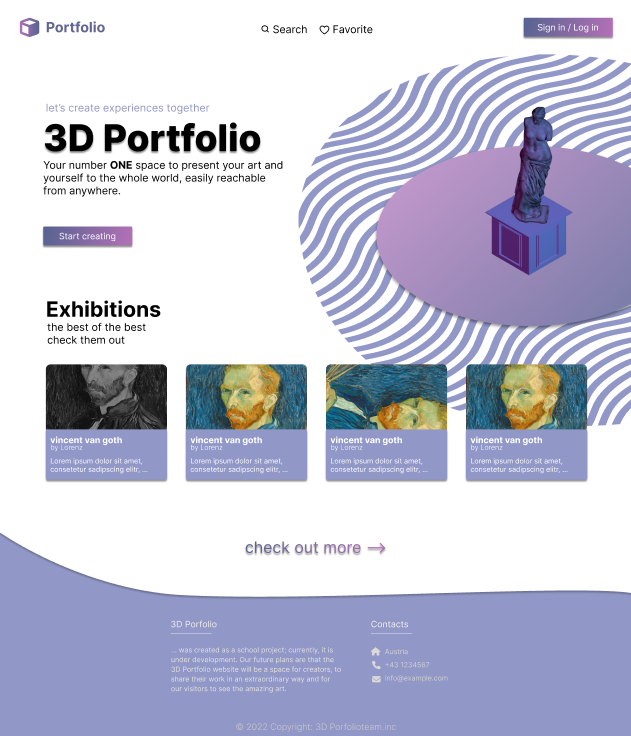
\includegraphics[scale=.5]{pics/startingpage.png}
    \caption{Landing Page}
    \label{fig:impl:finishedLandingpage}
\end{figure}

Um zwischen den verschiedenen Unterseiten der Webseite zu wechseln, wurde am oberen Bildschirmrand zusätzlich eine Navigationsleiste implementiert. Diese sogenannte Navbar besitzt je nach Unterseite verschiedene Designs. Diese ermöglicht ein angenehmes Navigieren auf jeder Seite (siehe \ref{lst:impl:routing}). Auch der Footer muss auf jeder Unterseite passend angezeigt werden. Um das Design von Navbar und Footer auf jeder Seite individuell zu gestalten, wird jeweils ein Service  in die entsprechende Komponente injiziert. Dadurch kann die Konfiguration am Design mit wenig Programmcode und Redundanz vorgenommen werden.

\subsection{Erledigte Userstories [L]}
\label{Finished Landingpage}
Bei der Fertigstellung der Landingpage wurden folgende Userstories vollendet: 
\begin{compactitem}
    \item Als erstmalige*r Besucher*in der Webseite möchte ich die benötigten Informationen über die Funktionen der Applikation verständlich erkennen können. Akzeptanzkriterien:
    Auf der Landingpage befinden sich:
    \begin{compactitem}
        \item Textstellen und Grafiken, die unser Projekt und die Funktionalitäten davon erklären
        \item Einen Call-To-Action (CTA) Button, der den User*in dazu einlädt, seine eigene Ausstellung zu erstellen. Beim Betätigen wird der Benutzer, falls er schon eingeloggt ist, weitergeleitet zum Editor, sonst zur Login Seite (hier gibt es die Möglichkeit, einen Account zu erstellen)
    \end{compactitem}
\end{compactitem}

